\documentclass[fin1, tisk]{fmfdelo}
%\documentclass[mat1, tisk]{fmfdelo}
% Če pobrišete možnost tisk, bodo povezave obarvane,
% na začetku pa ne bo praznih strani po naslovu, …

%%%%%%%%%%%%%%%%%%%%%%%%%%%%%%%%%%%%%%%%%%%%%%%%%%%%%%%%%%%%%%%%%%%%%%%%%%%%%%%
% METAPODATKI
%%%%%%%%%%%%%%%%%%%%%%%%%%%%%%%%%%%%%%%%%%%%%%%%%%%%%%%%%%%%%%%%%%%%%%%%%%%%%%%

% - vaše ime
\avtor{Peter Milivojević}

% - naslov dela v slovenščini
\naslov{Igre ustvarjanja omrežij}

% - naslov dela v angleščini
\title{Network creation games}

% - ime mentorja/mentorice s polnim nazivom:
%   - doc.~dr.~Ime Priimek
%   - izr.~prof.~dr.~Ime Priimek
%   - prof.~dr.~Ime Priimek
%   za druge variante uporabite ustrezne ukaze
\mentor{prof.~dr.~Sergio Cabello Justo}
% \somentor{...}
% \mentorica{...}
% \somentorica{...}
% \mentorja{...}{...}
% \somentorja{...}{...}
% \mentorici{...}{...}
% \somentorici{...}{...}

% - leto diplome
\letnica{2024} 

% - povzetek v slovenščini
%   V povzetku na kratko opišite vsebinske rezultate dela. Sem ne sodi razlaga
%   organizacije dela, torej v katerem razdelku je kaj, pač pa le opis vsebine.
\povzetek{...}

% - povzetek v angleščini
\abstract{...}

% - klasifikacijske oznake, ločene z vejicami
%   Oznake, ki opisujejo področje dela, so dostopne na strani https://www.ams.org/msc/
\klasifikacija{..., ...}

% - ključne besede, ki nastopajo v delu, ločene s \sep
\kljucnebesede{...\sep ...}

% - angleški prevod ključnih besed
\keywords{...\sep ...} % angleški prevod ključnih besed

% - angleško-slovenski slovar strokovnih izrazov
\slovar{
% \geslo{angleški izraz}{slovenski izraz}
% ...
}

% - ime datoteke z viri (vključno s končnico .bib), če uporabljate BibTeX
% \literatura{....bib}

%%%%%%%%%%%%%%%%%%%%%%%%%%%%%%%%%%%%%%%%%%%%%%%%%%%%%%%%%%%%%%%%%%%%%%%%%%%%%%%
% DODATNE DEFINICIJE
%%%%%%%%%%%%%%%%%%%%%%%%%%%%%%%%%%%%%%%%%%%%%%%%%%%%%%%%%%%%%%%%%%%%%%%%%%%%%%%

% naložite dodatne pakete, ki jih potrebujete
% \usepackage{...}
\usepackage{graphicx}
\usepackage{pgfplots}
\pgfplotsset{compat=1.17}

% deklarirajte vse matematične operatorje, da jih bo LaTeX pravilno stavil
% \DeclareMathOperator{\...}{...}

% vstavite svoje definicije ...
% \newcommand{\...}{...}

%%%%%%%%%%%%%%%%%%%%%%%%%%%%%%%%%%%%%%%%%%%%%%%%%%%%%%%%%%%%%%%%%%%%%%%%%%%%%%%
% ZAČETEK VSEBINE
%%%%%%%%%%%%%%%%%%%%%%%%%%%%%%%%%%%%%%%%%%%%%%%%%%%%%%%%%%%%%%%%%%%%%%%%%%%%%%%

\begin{document}

\title{Diplomska naloga: Igra ustvarjanja omrežja}
\author{Vaše ime}
\date{\today}
\maketitle

\section{Uvod}

Namen diplomske naloge je spoznati se z igrami ustvarjanja omrežja s poudarkom na dveh osnovnih verzijah tega problema.
V igri ustvarjanja omrežja imamo igralce, predstavljene kot vozlišča v grafu, ki želijo z 'sebično' izbiro svoje
strategije izboljšati svoj položaj. Običajno ima vsak igralec dva sebična cilja: minimizirati stroške
ustvarjanja povezav (omrežja) in minimizirati razdaljo do ostalih vozlišč (strošek uporabe omrežja).

V osnovnih igrah omrežij predpostavimo, da se ne da primerjati cene ustvarjanja in vzdrževanja povezav. Zato se
omejimo na že vnaprej podane grafe (omrežja), kjer lahko vozlišča (igralci) le zamenjajo svoje povezave ali v
posebnem primeru odstranijo povezavo, tako da zamenjajo povezavo za že obstoječo povezavo, s čimer se ena povezava
izbriše. Ukvarjali se bomo le z grafi brez zank in dvojnih povezav. Ne morejo pa ustvariti novih povezav.

\section{Teoretična podlaga}

Da bomo lahko razumeli obnašanje igralcev in lastnosti nastalih omrežij, bomo najprej obnovili teoretične temelje.
Ukvarjali se bomo izključno z povezanimi enostavnimi grafi.

\subsection{Osnovne definicije}

\begin{definicija}
Graf je urejen par \(G = (V, E)\), kjer je \(V\) neprazna množica točk grafa \(G\) in \(E\) množica povezav grafa \(G\), pri čemer je vsaka povezava par točk.
\end{definicija}

\begin{definicija}
Graf \(G\) je povezan, če za vsak par vozlišč \(u, v \in V(G)\) obstaja pot od \(u\) do \(v\).
\end{definicija}

\begin{definicija}
Naj bo \(G\) povezan graf in \(v \in V(G)\). Stopnja točke \(v\) je enaka vsoti števila povezav, ki imajo to točko za krajišče (in dvojnega števila zank v tej točki). Označimo jo z \(\deg(v)\).
\end{definicija}

\begin{definicija}
Naj bo \(G\) povezan graf in \(u, v \in V(G)\). Razdalja \(d(u, v)\) je dolžina najkrajše poti med vozliščema \(u\) in \(v\) v grafu \(G\).
\end{definicija}

\begin{definicija}
Naj bo \(G\) povezan graf. Premer grafa \(G\) je definiran kot \(\text{diam}(G) = \max_{u, v \in V(G)} d(u, v)\), kjer je \(d(u, v)\) razdalja med vozliščema \(u\) in \(v\) v grafu \(G\).
\end{definicija}

\begin{definicija}
Naj bo \(G\) povezan graf. Lokalni premer točke \(v\) grafa \(G\) je definiran kot \(\text{diam}(G) = \max_{u \in V(G)} d(u, v)\), kjer je \(d(u, v)\) razdalja med vozliščema \(u\) in \(v\) v grafu \(G\).
\end{definicija}

\begin{definicija}
Povezan graf \(G\) ima prerezno vozlišče \(v\), če graf \(G - v\) ni povezan.
\end{definicija}

\begin{definicija}
Naj bo \(G\) povezan graf z \(n\) vozlišči. Weinerjev indeks \(W = W(G)\) je definiran kot vsota vseh razdalj med vozlišči.
\[
W(G) = \sum_{i=1}^{n} \sum_{j=1}^{i} d_{ij} = \frac{1}{2} \sum_{i=1}^{n} \sum_{j=1}^{n} d_{ij}
\]
kjer \(d_{ij}\) označuje dolžino najkrajše poti med vozliščem \(i\) in \(j\).
\end{definicija}

\section{Igra}

Pomembno za razumevanje kasnejših delov diplomske naloge je tudi razumevanje, kaj je igra v smislu teorije iger.

\begin{definicija}
Strateška igra s funkcijo preferenc je trojica \((N, (A_i)_{i\in N}, (u_i)_{i\in N})\) pri čemer:
\begin{itemize}
    \item \(N\) je množica igralcev, v našem primeru je to število točk v grafu
    \item Za vsakega igralca \(i \in N\) je \(A_i\) neprazna množica njegovih akcij, med katerimi v danem trenutku izbira igralec \(i\)
    \item Za vsakega igralca \(i \in N\) je \(u_i\) funkcija preferenc na \(A_i\). Torej \(u_i : A_i \to \mathbb{R}\) v splošnem in \(u_i : A_i \to \mathbb{N}\) v našem primeru.
\end{itemize}
\end{definicija}

Za funkcijo preferenc lahko zapišemo sledeče relacije:

\(\forall a,b \in A_i\):
\begin{itemize}
    \item \(u(a) \geq u(b) \Rightarrow a\) je vsaj tako dobro kot \(b\)
    \item \(u(a) > u(b) \Rightarrow a\) je boljše kot \(b\)
    \item \(u(a) = u(b) \Rightarrow\) igralec \(i\) je indiferenten med \(a\) in \(b\)
\end{itemize}

\section{Ravnovesje}

V tem delu bomo definirali pravila igre in pogoje za nastanek ravnovesij.

\begin{definicija}
Graf je v \textit{ravnotežju glede na vsoto razdalj}, če za vsako povezavo \(vw\) in za vsako vozlišče \(w'\) zamenjava povezave \(vw\) z povezavo \(vw'\) ne zmanjša celotne vsote razdalj od vozlišča \(v\) do vseh ostalih vozlišč.
\end{definicija}

\begin{definicija}
Graf je v \textit{ravnotežju glede na maksimalno razdaljo}, če za vsako povezavo \(vw\) in za vsako vozlišče \(w'\) zamenjava povezave \(vw\) z povezavo \(vw'\) ne zmanjša lokalnega premera vozlišča \(v\). Nadalje odstranitev povezave \(vw\) poveča lokalni premer vozlišča \(v\).
\end{definicija}

\begin{definicija}
Naj bo \(G\) povezan graf. Graf \(G\) je \textit{kritičen za odstranitev povezave}, če odstranitev katere koli povezave \(uv \in E(G)\) poveča lokalni premer vozlišča \(v\) in vozlišča \(u\).
\end{definicija}

\begin{definicija}
Naj bo \(G\) povezan graf. Graf \(G\) je \textit{stabilen za dodajanje povezave}, če dodajanje katere koli povezave \(uv \in E(G)\) ne zmanjša lokalnega premera vozlišča \(v\) in vozlišča \(u\).
\end{definicija}

\section{Cena anarhije in cena stabilnosti}

Ukvarjali se bomo tudi s ceno anarhije (PoA) in ceno stabilnosti (PoS). Ti ceni merita, kako se učinkovitost sistema poslabša zaradi sebičnega vedenja njegovih agentov.

\begin{definicija}
Cena anarhije je razmerje med vrednostjo najslabšega ravnovesja in optimalno socialno ceno.
\[
PoA = \frac{\text{Socialna cena najslabšega ravnovesja}}{\text{Socialna cena optimalne postavitve}} = \frac{\max_{G\in R} SC(G)}{\min_{G\in A} SC(G)}
\]
\end{definicija}

\begin{definicija}
Cena stabilnosti je razmerje med najboljšo socialno ceno ravnovesja in optimalno socialno ceno.
\[
PoS = \frac{\text{Socialna cena najboljšega ravnovesja}}{\text{Socialna cena optimalne postavitve}} = \frac{\min_{G\in R} SC(G)}{\min_{G\in A} SC(G)}
\]
\end{definicija}

Kjer \(A\) predstavlja množico vseh možnih povezanih grafov z \( |V(G)| = n \) vozlišči in največ \( |E(G)| = m \) povezavami. Množica \(R \subseteq A\) pa predstavlja množico vseh ravnovesnih grafov, ki lahko nastanejo iz začetnih grafov z \(n\) vozlišči in \(m\) povezavami.

\section{Teoretični del diplomske naloge}

Nekoliko zahtevnejši in bolj raznoliki grafi od polnih grafov so drevesa.

\begin{izrek}
Če je ravnovesni graf za skupno vsoto razdalj v preprosti igri ustvarjanja omrežja drevo, potem ima premer največ 2 in je kot tak zvezda.
\end{izrek}

\begin{dokaz}
Dokaza se bomo lotili z protislovjem. Predpostavimo, da je ravnovesni graf drevo s premerom 3 ali več. Ker ima premer vsaj 3, obstajata vozlišči \(u\) in \(v\) oddaljeni eno od druge za točno 3 preko najkrajše in edine poti, ki gre skozi dve točki, ki jih označimo z \(a\) in \(b\). Tako imamo pot \(v \to a \to b \to u\). Z \(s_v, s_a, s_b, s_u\) označimo število morebitnih točk poddreves upetih na \(v, a, b, u\). Obravnavamo dve možni zamenjavi:
\end{dokaz}

\begin{figure}[h]
    \centering
    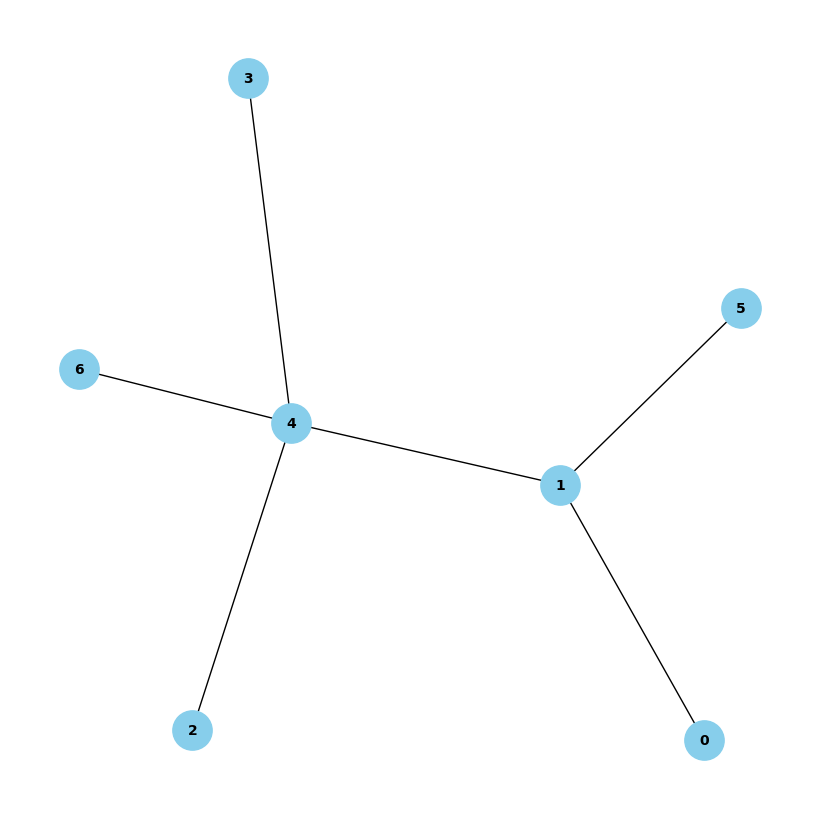
\includegraphics[width=0.3\textwidth]{drevo_1.png}
    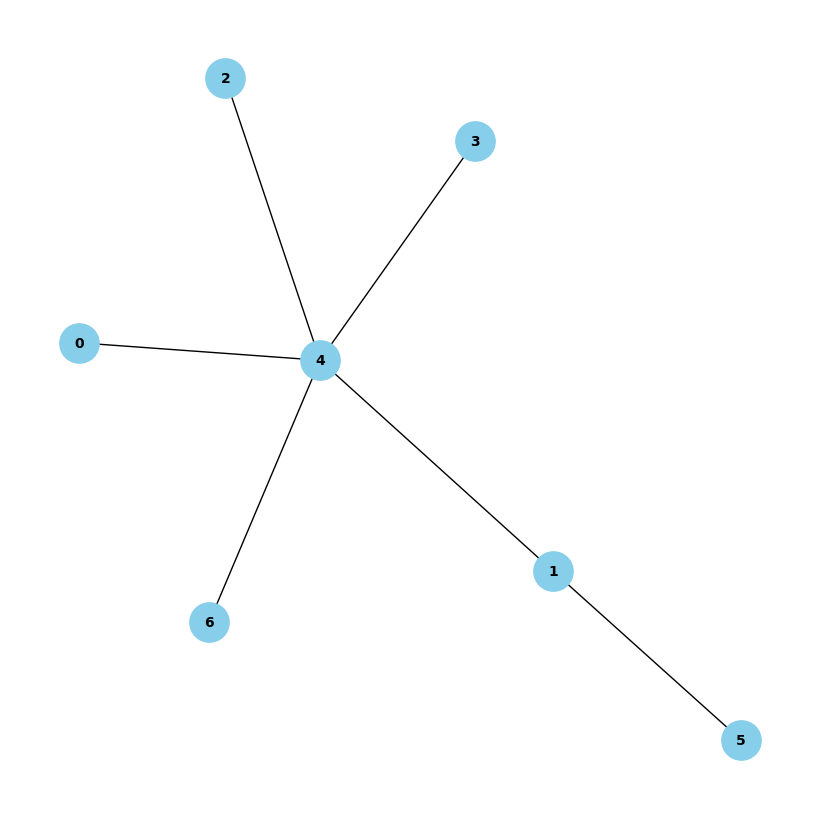
\includegraphics[width=0.3\textwidth]{drevo_2.png}
    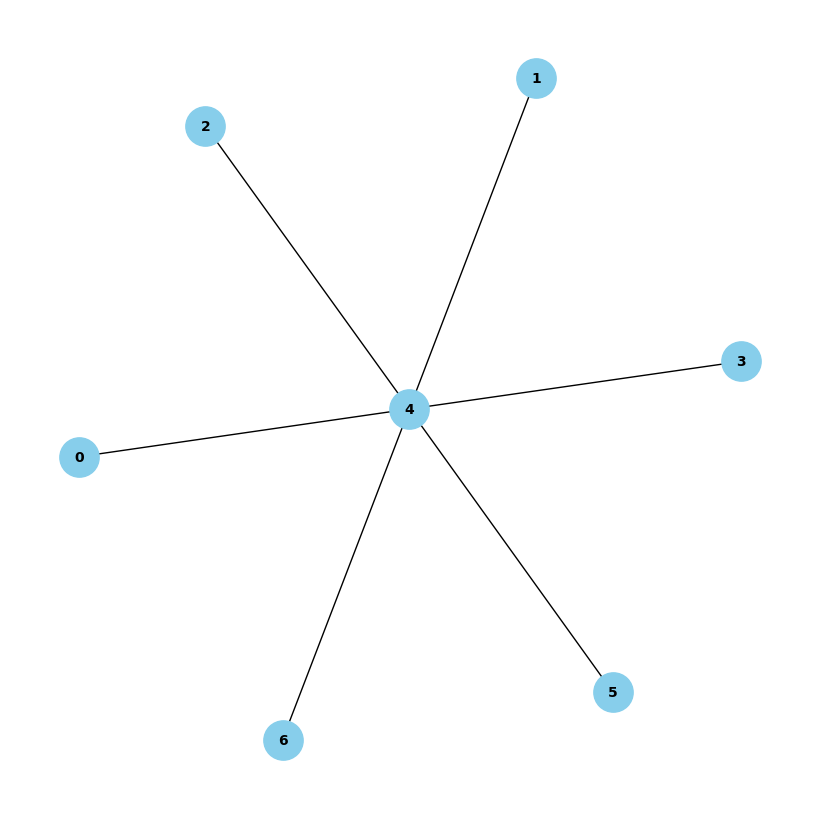
\includegraphics[width=0.3\textwidth]{drevo_3.png}
    \caption{Ilustracije dreves}
\end{figure}

\begin{lema}
V vsakem ravnovesnem grafu igre maksimalne razdalje se lokalni premer za kateri koli dve poljubni vozlišči razlikuje največ za 1.
\end{lema}

\begin{dokaz}
Predpostavimo, da je graf v \textit{ravnotežju glede na maksimalno razdaljo} in ima vozlišče \(v\) z lokalnim premerom \(d\) in vozlišče \(w\) z lokalnim premerom vsaj \(d+2\). Naj bo \(T\) drevo, ki ga dobimo z iskanjem v širino iz vozlišča \(v\). Vozlišče \(w\) z zamenjavo svoje povezave s staršem v \(T\) z povezavo do \(v\) (korena \(T\)) zmanjša svoj lokalni premer. Opazimo, da ta zamenjava lahko le zmanjša ali ohrani globine vozlišč v \(T\), zato lokalni premer vozlišča \(v\) ostane največ \(d\). Tako se lokalni premer vozlišča \(w\) zmanjša na vsaj \(d+1\), saj se \(w\) lahko premakne po novo nastali povezavi \(wv\) do \(v\) in nato sledi poti \(v\) do vseh ostalih vozlišč. Ta zamenjava je v nasprotju s predpostavko, da je graf v \textit{ravnotežju glede na maksimalno razdaljo}, saj lahko vozlišče \(u\) izboljša svoj položaj (zmanjša svoj lokalni premer) z omenjeno zamenjavo povezav.
\end{dokaz}

\begin{lema}
Če ima ravnovesni graf za maksimalno razdaljo prerezno vozlišče \(v\), potem ima lahko samo ena izmed povezanih komponent \(G - v\) vozlišče z razdaljo več kot 1 od \(v\).
\end{lema}

\begin{dokaz}
Ponovno bomo dokazali lemo z protislovjem. Naj bo \(d\) lokalni premer prereznega vozlišča \(v\) in naj bo vozlišče \(u\) na razdalji \(d\) od \(v\). Z \(U\) označimo povezano komponento \(G - v\), ki vsebuje \(u\). Predpostavimo, da \(G - U\) vsebuje vozlišče \(z\), ki je za več kot 1 oddaljeno od vozlišča \(v\). Ker je vozlišče \(v\) prerezno in \(z\) in \(u\) nista vozlišči iste povezane komponente \(G - v\), mora vsaka pot med njima prečkati \(v\). Tako je najkrajša pot od \(z\) do \(u\) dolga \(d + 2\). Lokalni premer \(z\) in \(u\) je zato vsaj \(d + 2\), kar se za več kot 1 razlikuje od lokalnega premera vozlišča \(v\), in je tako v nasprotju z predhodno lemo. Zato graf, ki ima več kot eno povezano komponento \(G - v\) z vozliščem z razdaljo več kot 1 od \(v\), ne more biti ravnovesni graf.
\end{dokaz}

\begin{izrek}
Če je ravnovesni graf za maksimalno razdaljo drevo, potem ima premer največ 3.
\end{izrek}

\begin{dokaz}
Predpostavimo, da je ravnovesni graf za maksimalno razdaljo drevo in ima premer vsaj 4. Potem obstajata vozlišči \(v\) in \(u\), ki sta na razdalji točno 4 in med njima obstaja pot dolžine 4: \(v \to a \to b \to c \to u\). Ker je graf drevo, je vozlišče \(b\) prerezno vozlišče z dvema povezanima komponentama \(G - b\), ki vsebujeta vozlišči \(v\) in \(u\), ki sta na razdalji več kot 1 od \(b\), in tako v protislovju z predhodno lemo.
\end{dokaz}

\begin{lema}
Za vozlišče \(v\) z lokalnim premerom 2 zamenjava sosednje povezave ne izboljša vsote razdalj od \(v\) do vseh ostalih vozlišč. Prav tako tudi svojega lokalnega premera ne more izboljšati.
\end{lema}

\begin{dokaz}
Naj ima graf \(G\) \(n\) vozlišč in naj ima poljubno vozlišče z lokalnim premerom 2 stopnjo \(\deg(v) = k\). Tako ima vozlišče \(v\) \(k\) sosednjih vozlišč in \(n - k - 1\) vozlišč na razdalji 2, saj je lokalni premer \(v\) enak 2. Vsota razdalj od \(v\) do vseh ostalih vozlišč je zato \(1 \cdot k + 2 \cdot (n - k - 1)\). Vozlišče \(v\) z menjavo poljubne povezave ne spremeni števila sosednjih vozlišč \(k\). Zamenjavo ene izmed povezav vozlišča \(v\) lahko obravnavamo kot odstranitev ene obstoječe povezave, s katero se izgubi eno sosednje vozlišče, in dodajo nove povezave, s katero se pridobi eno sosednje vozlišče. Tako ima vozlišče \(v\), ne glede na zamenjavo povezav, \(k\) sosednjih vozlišč in \(n - k - 1\) vozlišč na razdalji vsaj 2, saj se razdalja do ne sosednjega vozlišča lahko le poveča ali ostane enaka 2. Zato je vsota razdalj od \(v\) do vseh ostalih vozlišč po zamenjavah povezav \(v\) enaka ali večja od \(1 \cdot k + 2 \cdot (n - k - 1)\).
\end{dokaz}

\begin{posledica}
Vsak graf z premerom 2 ali manj je v \textit{ravnotežju glede na vsoto razdalj} in hkrati socialni optimum.
\end{posledica}

\begin{posledica}
Cena stabilnosti je 1.
\end{posledica}

\begin{izrek}
Naj bo \(G\) graf z \(n\) vozlišči in \(m\) povezavami, potem je \(W(G) = n^2 - n - m\), če in samo če je premer grafa 2 ali manj.
\end{izrek}

\begin{dokaz}
Predpostavimo, da je \(G\) graf reda \(n\) in velikosti \(m\) ter da velja \(\text{diam}(G) \leq 2\). Definirajmo množici \(A = \{u \in V | e(u) = 1\}\) in \(B = \{u \in V | e(u) = 2\}\). Potem velja \(|A| + |B| = n\). Če je \(u \in A\), potem je \(d(u) = n - 1\) (vsota vseh razdalj od \(u\) do ostalih vozlišč), in če je \(u \in B\), definiramo dve množici \(B_1\) in \(B_2\) kot \(B_1 = \{v \in V | d(u, v) = 1\}\) in \(B_2 = \{v \in V | d(u, v) = 2\}\).

Nato velja:
\begin{align*}
d(u) &= |B_1| + 2|B_2| \\
&= |B_1| + |B_2| + |B_2| \\
&= n - 1 + (n - 1 - |B_1|) \\
&= 2n - 2 - |B_1| \\
&= 2n - 2 - \deg(u)
\end{align*}

In zato sledi:
\begin{align*}
W(G) &= \frac{1}{2} \sum_{u \in V} d(u) \\
&= \frac{1}{2}( \sum_{u \in A} d(u) + \sum_{u \in B} d(u)) \\
&= \frac{1}{2}( (n - 1)|A| + \sum_{u \in B} 2n - 2 - \deg(u)) \\
&= \frac{1}{2}( (n - 1)|A| + (2n - 2)|B| - \sum_{u \in B} \deg(u)) \\
&= \frac{1}{2}( (n - 1)(|A| + |B|) + (n - 1)|B| - \sum_{u \in B} \deg(u)) \\
&= \frac{1}{2}( (n - 1)n + (n - 1)(n - |A|) - \sum_{u \in B} \deg(u)) \\
&= \frac{1}{2}( (n - 1)n + (n - 1)n - (n - 1)|A| - \sum_{u \in B} \deg(u)) \\
&= \frac{1}{2}( 2(n - 1)n  - \sum_{u \in V} \deg(u)) \\
&= \frac{1}{2}( 2(n - 1)n  - 2m) \\
&= n^2 - n - m
\end{align*}

Kar dokaže, da je \(W(G) = n^2 - n - m\) za grafe s premerom manjšim od 2 (\(\text{diam}(G) \leq 2\)). V drugem delu bomo dokazali, da ta enakost ne velja za grafe s premerom večjim od 2. Za graf \(G\), ki ima premer vsaj 3 (\(\text{diam}(G) \geq 3\)), bomo definirali množici \(A = \{u \in V | e(u) = 2\}\) in \(B = \{u \in V | e(u) \geq 3\}\). Za kateri velja \(|A| + |B| = n\). Če je \(u \in A\), potem iz zgoraj dokazanega velja \(d(u) = 2n - 2 - \deg(u)\). Za \(u \in B\) pa bomo definirali sledeče tri podmnožice:

\begin{align*}
B_1 &= \{v \in V | d(u,v) = 1\}, \\
B_2 &= \{v \in V | d(u,v) = 2\}, \\
B_3 &= \{v \in V | d(u,v) \geq 3\}. \\
\text{Očitno, } |B_1| + |B_2| + |B_3| &= n - 1. \\
d(u) &\geq |B_1| + 2|B_2| + 3|B_3| \\
&= |B_1| + |B_2| + |B_3| + |B_2| + 2|B_3| \\
&= n - 1+ (n - 1 - |B_1|)+ | B_3| \\
&= 2n-2-\deg(u) + | B_3| \\
&= 2n-2-\deg(u) + | B_3| \\
&\geq 2n-2-\deg(u)+1 \\
&\geq 2n-1-\deg(u). \\
\therefore W(G) &= \frac{1}{2} \sum_{u \in V} d(u) \\
&=\frac{1}{2}(\sum_{u \in A} d(u) + \sum_{u \in B} d(u)) \\
&\geq \frac{1}{2}((\sum_{u \in A} (2n-2-\deg(u))+(\sum_{u \in B} (2n-1-\deg(u))) \\
&=\frac{1}{2}((2n-2)(|A| + |B|) - \sum_{u \in A} \deg(u))-(\sum_{u \in B} \deg(u))+ |B|) \\
&=\frac{1}{2}((2n-2)n - (\sum_{u \in V} \deg(u)) + |B|) \\
&=\frac{1}{2}(2(n-1)n - 2m + |B|) \\
&=n(n - 1) - m + \frac{1}{2}|B| \\
&\geq n(n - 1) - m + 1
\end{align*}
\end{dokaz}

\begin{posledica}
Za vsak graf \(G\) z \(n\) vozlišči, \(m\) povezavami in premerom večjim od 2 velja:
\[
W(G) \geq n^2 - n - m + 1.
\]
Enačaj velja, kadar ima graf \(G\) natanko dve vozlišči z lokalnim premerom 3 in vsa ostala vozlišča z lokalnim premerom 2.
\end{posledica}

\begin{izrek}
Obstaja ravnovesni graf za skupno vsoto razdalj s premerom 3.
\end{izrek}

\begin{dokaz}
Graf na spodnji sliki ima premer 3 in je v \textit{ravnotežju glede na vsoto razdalj}. Točke 1, 3, 5 in 7 imajo lokalni premer 2 in tako po predhodni lemi ne morejo same zmanjšati svoje vsote razdalj do vseh ostalih vozlišč. Točke 2, 4, 6 in 8 so simetrične in celo povezave teh točk so simetrične, zato je dovolj pogledati vse možne zamenjave le za eno izmed povezav teh točk. Točka 2 ima vsoto razdalj do vseh ostalih točk enako 1 + 1 + 2 + 2 + 2 + 2 + 3 = 13. Za preverjanje ali lahko točka 2 izboljša svoj položaj bomo poskusili z zamenjavo povezave med točkama 2 in 1 z novimi povezavami med točko 2 in ostalimi povezavami. Če povezavo 21 zamenjamo s povezavo 24, ima vozlišče 2 vsoto razdalj enako 1 + 1 + 2 + 2 + 3 + 3 + 3 = 15. Če povezavo 21 zamenjamo s povezavo 25, ima vozlišče 2 vsoto razdalj enako 1 + 1 + 2 + 2 + 2 + 2 + 3 = 13. Če povezavo 21 zamenjamo s povezavo 26, ima vozlišče 2 vsoto razdalj enako 1 + 1 + 2 + 2 + 2 + 3 + 3 = 14. Če povezavo 21 zamenjamo s povezavo 27, ima vozlišče 2 vsoto razdalj enako 1 + 1 + 2 + 2 + 2 + 3 + 3 = 14. Če povezavo 21 zamenjamo s povezavo 28, ima vozlišče 2 vsoto razdalj enako 1 + 1 + 2 + 2 + 2 + 3 + 3 = 13.
\end{dokaz}

\begin{figure}[h]
    \centering
    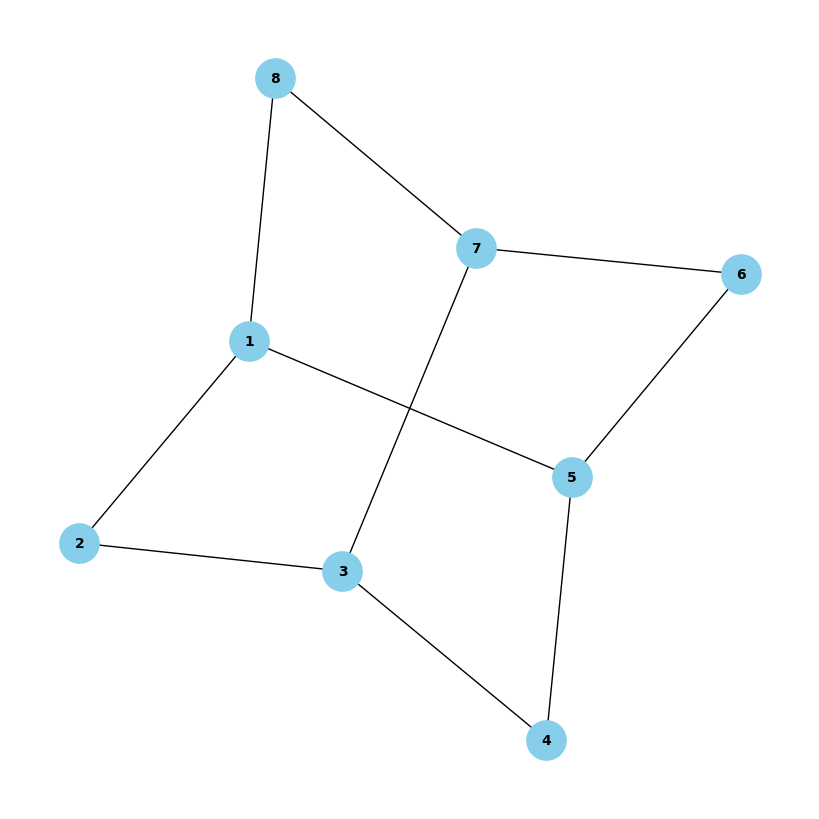
\includegraphics[width=0.9\textwidth]{vsota_premer_3.png}
    \caption{Graf s premerom 3}
\end{figure}

\begin{izrek}
Vsak ravnovesni graf za skupno vsoto razdalj ima premer \(2^{O(\sqrt{\lg n})}\).
\end{izrek}

\begin{lema}
Vsak ravnovesni graf za skupno vsoto razdalj ima premer največ \(2 \lg n\) ali za vsako vozlišče \(v\) obstaja povezava \(xy\), kjer je \(d(u, x) \leq \lg n\) in zamenjava povezave \(xy\) zmanjša vsoto razdalj od \(x\) za največ \(2n(1 + \lg n)\).
\end{lema}

\begin{lema}
V vsakem ravnovesnem grafu za skupno vsoto razdalj dodajanje poljubne povezave \(uv\) zmanjša vsoto razdalj od \(u\) za največ \(5n \log n\).
\end{lema}

\begin{izrek}
Obstaja ravnovesni graf za maksimalno razdaljo s premerom \(\Theta(\sqrt{n})\).
\end{izrek}

\begin{figure}[h]
    \centering
    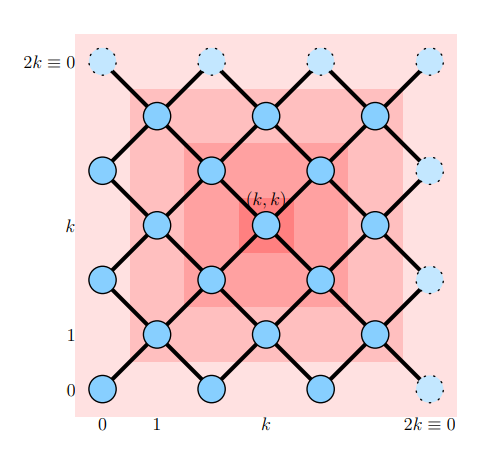
\includegraphics[width=0.9\textwidth]{Plagiat.png}
    \caption{Ravnovesni graf za maksimalno razdaljo}
\end{figure}

\begin{izrek}
Vsak ravnovesni graf za skupno vsoto razdaljo \(G\) z \(n \geq 24\) vozlišči in premerom \(d > 2 \lg n\) inducira podgraf z \(\epsilon\)-skoraj-enotno-razdaljo \(G'\) z \(n\) vozlišči in premerom \(\Theta\left(\frac{\varepsilon d}{\lg n}\right)\) in podgraf z \(\epsilon\)-enotno-razdaljo \(G'\) z \(n\) vozlišči in premerom \(\Theta\left(\frac{\varepsilon d}{\lg^2 n}\right)\).
\end{izrek}

\begin{izrek}
Vsak ravnovesni graf za osnovne igre ustvarjanja omrežij (morda samo za vsoto) ima največ eno po povezavah 2-povezano komponento.
\end{izrek}

\section{Testiranje}

V razdelku Testiranje smo s pomočjo programskega jezika Python podrobneje spoznali igre ustvarjanja omrežij, grafe, ki v takih igrah nastajajo, in preverjali nekatere domneve o ravnovesnih grafih.

Najprej smo primerjali število različnih ravnovesnih grafov med ravnovesnimi grafi glede na vsoto, ravnovesnimi grafi glede na razdaljo in grafi, ki so hkrati stabilni za dodajanje povezav in kritični za odstranitev povezav.

Po pričakovanjih smo opazili, da je bilo največ ravnovesnih grafov glede na vsoto in najmanj kritičnih in stabilnih hkrati. Opazili smo tudi, da pri določenih kombinacijah števila vozlišč in števila povezav ravnovesni grafi glede na razdaljo ne obstajajo.

V nadaljevanju smo si ogledali nekaj različnih algoritmov za iskanje ravnovesnega grafa glede na največjo razdaljo in koliko od najdenih ravnovesnih grafov pri posameznem algoritmu je dreves.

Pogledali smo si tudi katera točka v drevesnih grafih pri igri doseže najboljšo pozicijo tako v igri, kjer imajo vse povezave enako ceno, kot tudi v igri v realni ravnini.

\begin{table}[h]
    \centering
    \scriptsize
    \begin{tabular}{lllll}
        Vozlišča & Povezave & SUM & MAX & Kritično \\ 
        \hline
        2 & 1 & 1 & 1 & 1 \\ 
        3 & 2 & 1 & 1 & 0 \\ 
        3 & 3 & 1 & 1 & 1 \\ 
        4 & 3 & 1 & 1 & 1 \\ 
        4 & 4 & 2 & 1 & 0 \\ 
        4 & 5 & 1 & 0 & 0 \\ 
        4 & 6 & 1 & 1 & 1 \\ 
        5 & 4 & 1 & 1 & 1 \\ 
        5 & 5 & 2 & 1 & 1 \\ 
        5 & 6 & 4 & 1 & 0 \\ 
        5 & 7 & 4 & 0 & 0 \\ 
        5 & 8 & 2 & 0 & 0 \\ 
        5 & 9 & 1 & 0 & 0 \\ 
        5 & 10 & 1 & 1 & 1 \\ 
        6 & 5 & 1 & 2 & 1 \\ 
        6 & 6 & 1 & 1 & 1 \\ 
        6 & 7 & 3 & 1 & 1 \\ 
        6 & 8 & 10 & 1 & 0 \\ 
        6 & 9 & 15 & 1 & 1 \\ 
        6 & 10 & 12 & 0 & 0 \\ 
        6 & 11 & 9 & 0 & 0 \\ 
        6 & 12 & 5 & 0 & 0 \\ 
        6 & 13 & 2 & 0 & 0 \\ 
        6 & 14 & 1 & 0 & 0 \\ 
        6 & 15 & 1 & 1 & 1 \\ 
        7 & 6 & 1 & 2 & 1 \\ 
        7 & 7 & 1 & 3 & 1 \\ 
        7 & 8 & 2 & 0 & 0 \\ 
        7 & 9 & 8 & 3 & 3 \\ 
        7 & 10 & 24 & 2 & 1 \\ 
        7 & 11 & 52 & 0 & 0 \\ 
        7 & 12 & 76 & 1 & 1 \\ 
        7 & 13 & 75 & 0 & 0 \\ 
        7 & 14 & 57 & 0 & 0 \\ 
        7 & 15 & 38 & 0 & 0 \\ 
        7 & 16 & 21 & 0 & 0 \\ 
        7 & 17 & 10 & 0 & 0 \\ 
        7 & 18 & 5 & 0 & 0 \\ 
        7 & 19 & 2 & 0 & 0 \\ 
        7 & 20 & 1 & 0 & 0 \\ 
        7 & 21 & 1 & 1 & 1 \\ 
        8 & 7 & 1 & 3 & 1 \\ 
        8 & 8 & 1 & 3 & 2 \\ 
        8 & 9 & 2 & 1 & 1 \\ 
        8 & 10 & 7 & 4 & 2 \\ 
        8 & 11 & 15 & 4 & 3 \\ 
        8 & 12 & 55 & 4 & 3 \\ 
        8 & 13 & 165 & 2 & 2 \\ 
        8 & 14 & 387 & 0 & 0 \\ 
        8 & 15 & 649 & 1 & 1 \\ 
        8 & 16 & 787 & 1 & 1 \\ 
        8 & 17 & 733 & 0 & 0 \\ 
        8 & 18 & 567 & 0 & 0 \\ 
        8 & 19 & 370 & 0 & 0 \\ 
        8 & 20 & 211 & 0 & 0 \\ 
        8 & 21 & 111 & 0 & 0 \\ 
        8 & 22 & 56 & 0 & 0 \\ 
        8 & 23 & 24 & 0 & 0 \\ 
        8 & 24 & 11 & 0 & 0 \\ 
        8 & 25 & 5 & 0 & 0 \\ 
        8 & 26 & 2 & 0 & 0 \\ 
        8 & 27 & 1 & 0 & 0 \\ 
        8 & 28 & 1 & 1 & 1 \\ 
    \end{tabular}
    \caption{Število različnih ravnovesnih grafov glede na vsoto, maksimalno razdaljo in kritičnost za odstranitve povezav}
\end{table}

\begin{table}[h]
    \centering
    \begin{tabular}{llll}
        Št. vozlišč & SUM  & MAX & krit\\
        \hline
        2           & 1    & 1   & 1   \\
        3           & 2    & 2   & 1   \\
        4           & 5    & 3   & 2   \\
        5           & 15   & 4   & 3   \\
        6           & 60   & 7   & 5   \\
        7           & 374  & 12  & 8   \\
        8           & 4161 & 24  & 17 
    \end{tabular}
    \caption{Strnjeno po vozliščih}
\end{table}

Zanimal nas je tudi socialni optimum za maksimalno verzijo in ali je hkrati tudi ravnovesje.

\begin{table}[h]
    \centering
    \begin{tabular}{|c|*{16}{c|}}
    \hline
    \multirow{\textbf{n$\backslash$e}} & \multicolumn{16}{c|}{\textbf{Število povezav}} \\ \cline{2-17}
    & \textbf{n - 1} & \textbf{n} & \textbf{n + 1} & \textbf{n + 2} & \textbf{n + 3} & \textbf{n + 4} & \textbf{n + 5} 
    & \textbf{n + 6} & \textbf{n + 7} & \textbf{n + 8} & \textbf{n + 9} & \textbf{n + 10} & \textbf{n + 11} & \textbf{n + 12} 
    & \textbf{n + 13} & \textbf{n + 14}\\
    \hline
        2 & (2, 'Je')  &            &            &            &            &            &            &            &            &            &            &            &            &            &           &           \\
        3 & (5, 'Je')  & (3, 'Je')  &            &            &            &            &            &            &            &            &            &            &            &            &           &           \\
        4 & (7, 'Je')  & (7, 'Ni')  & (6, 'Ni')  & (4, 'Je')  &            &            &            &            &            &            &            &            &            &            &           &           \\
        5 & (9, 'Je')  & (9, 'Ni')  & (9, 'Ni')  & (8, 'Ni')  & (8, 'Ni')  & (7, 'Ni')  & (5, 'Je')  &            &            &            &            &            &            &            &           &           \\
        6 & (11, 'Je') & (11, 'Ni') & (11, 'Ni') & (11, 'Ni') & (10, 'Ni') & (10, 'Ni') & (10, 'Ni') & (9, 'Ni')  & (9, 'Ni')  & (8, 'Ni')  & (6, 'Je')  &            &            &            &           &           \\
        7 & (13, 'Je') & (13, 'Ni') & (13, 'Ni') & (13, 'Ni') & (13, 'Ni') & (12, 'Ni') & (12, 'Ni') & (12, 'Ni') & (12, 'Ni') & (11, 'Ni') & (11, 'Ni') & (11, 'Ni') & (10, 'Ni') & (10, 'Ni') & (9, 'Ni') & (7, 'Je') \\
    \hline
    \end{tabular}
    \caption{Socialni optimum za maximalno verzijo}
\end{table}

\section{Algoritmi}

V tem besedilu bomo opisali štiri algoritme za optimizacijo grafov v latex kodi.

\subsection*{Swap Remove}
Algoritem \texttt{swap\_remove} iterativno preizkuša različne povezave med vozlišči v grafu z namenom zmanjšanja ekscentričnosti vozlišč. Pri tem odstrani obstoječe povezave in doda nove, če se ekscentričnost zmanjša, hkrati pa ohranja povezanost grafa.

\subsection*{Remove Add}
Algoritem \texttt{remove\_add} preizkuša odstranitev obstoječih povezav v grafu in oceni vpliv na ekscentričnost vozlišč. Če se ekscentričnost ne poveča ali se zmanjša, obdrži spremembo. Nato poskuša dodati nove povezave med vozlišči, če to še dodatno zmanjša ekscentričnost.

\subsection*{Swap All Remove}
Algoritem \texttt{swap\_all\_remove} sistematično preizkuša zamenjavo obstoječih povezav z novimi in oceni vpliv na ekscentričnost vozlišč. V drugi fazi odstranjuje povezave in preverja, ali se ekscentričnost zmanjša, hkrati pa zagotavlja, da graf ostane povezan.

\subsection*{Remove All Add}
Algoritem \texttt{remove\_all\_add} najprej odstrani obstoječe povezave v grafu in oceni vpliv na ekscentričnost vozlišč. Nato poskuša dodati nove povezave, ki dodatno zmanjšajo ekscentričnost, pri tem pa ves čas ohranja povezanost grafa.

\begin{table}[h]
    \centering
    \scriptsize
    \begin{tabular}{|l|l|l|l|l|l|l|}
    \hline
        Vsi grafi & s\_r & r\_a & sa\_r & ra\_a & Vozlišča & Povezave \\ 
        \hline
        1 & 1 & 1 & 1 & 1 & 2 & 1 \\ 
        3 & 3 & 3 & 3 & 3 & 3 & 2 \\ 
        1 & 0 & 0 & 0 & 0 & 3 & 3 \\ 
        16 & 16 & 16 & 16 & 16 & 4 & 3 \\ 
        15 & 12 & 12 & 12 & 12 & 4 & 4 \\ 
        6 & 6 & 6 & 6 & 6 & 4 & 5 \\ 
        1 & 0 & 0 & 0 & 0 & 4 & 6 \\ 
        125 & 125 & 125 & 125 & 125 & 5 & 4 \\ 
        222 & 204 & 204 & 201 & 210 & 5 & 5 \\ 
        205 & 175 & 175 & 175 & 175 & 5 & 6 \\ 
        120 & 109 & 109 & 109 & 109 & 5 & 7 \\ 
        45 & 42 & 42 & 42 & 42 & 5 & 8 \\ 
        10 & 10 & 10 & 10 & 10 & 5 & 9 \\ 
        1 & 0 & 0 & 0 & 0 & 5 & 10 \\ 
        1296 & 1296 & 1296 & 1296 & 1296 & 6 & 5 \\ 
        3660 & 3488 & 3500 & 3470 & 3540 & 6 & 6 \\ 
        5700 & 4948 & 5023 & 4844 & 5160 & 6 & 7 \\ 
        6165 & 5166 & 5284 & 4842 & 5278 & 6 & 8 \\ 
        4945 & 4136 & 4209 & 4037 & 4251 & 6 & 9 \\ 
        2997 & 2621 & 2647 & 2585 & 2666 & 6 & 10 \\ 
        1365 & 1249 & 1255 & 1240 & 1265 & 6 & 11 \\ 
        455 & 429 & 429 & 429 & 431 & 6 & 12 \\ 
        105 & 99 & 99 & 99 & 99 & 6 & 13 \\ 
        15 & 15 & 15 & 15 & 15 & 6 & 14 \\ 
        1 & 0 & 0 & 0 & 0 & 6 & 15 \\ 
        16807 & 16807 & 16807 & 16807 & 16807 & 7 & 6 \\ 
        68295 & 56683 & 57681 & 47098 & 62565 & 7 & 7 \\ 
        156555 & 119891 & 122033 & 125319 & 126906 & 7 & 8 \\ 
        258125 & 190438 & 193894 & 207053 & 187011 & 7 & 9 \\ 
        331506 & 245268 & 250974 & 255672 & 231233 & 7 & 10 \\ 
        343140 & 261988 & 268460 & 261386 & 245093 & 7 & 11 \\ 
        290745 & 230004 & 235253 & 228026 & 219692 & 7 & 12 \\ 
        202755 & 166522 & 169358 & 164950 & 163127 & 7 & 13 \\ 
        116175 & 99175 & 100329 & 98291 & 99190 & 7 & 14 \\ 
        54257 & 48056 & 48424 & 47701 & 48619 & 7 & 15 \\ 
        20349 & 18631 & 18708 & 18550 & 18907 & 7 & 16 \\ 
        5985 & 5619 & 5627 & 5612 & 5684 & 7 & 17 \\ 
        1330 & 1267 & 1267 & 1267 & 1273 & 7 & 18 \\ 
        210 & 200 & 200 & 200 & 200 & 7 & 19 \\ 
        21 & 21 & 21 & 21 & 21 & 7 & 20 \\ 
        1 & 0 & 0 & 0 & 0 & 7 & 21 \\ 
    \end{tabular}
    \caption{Rezultati algoritmov za optimizacijo grafov}
\end{table}

Tukaj so strnjeni rezultati po vozliščih.

\begin{table}[h]
    \centering
    \scriptsize
    \begin{tabular}{|l|l|l|l|l|l|l|}
    \hline
        Vsi grafi & s\_r & r\_a & sa\_r & ra\_a & Vozlišča & ~ \\ 
        \hline
        1 & 1 & 1 & 1 & 1 & 2 & ~ \\ 
        4 & 3 & 3 & 3 & 3 & 3 & ~ \\ 
        38 & 34 & 34 & 34 & 34 & 4 & ~ \\ 
        728 & 665 & 665 & 662 & 671 & 5 & ~ \\ 
        26704 & 23447 & 23757 & 22857 & 24001 & 6 & ~ \\ 
        1866256 & 1460570 & 1489036 & 1477953 & 1426328 & 7 & ~ \\ 
    \end{tabular}
    \caption{Strnjeni rezultati po vozliščih}
\end{table}

\section{Optimalno pozicioniranje na tržišču}

Pri igri vsote smo uporabili dva podobna algoritma za iskanje ravnovesja. Oba algoritma delujeta tako, da prva točka v grafu optimizira svoj položaj glede na stanje ostalih točk, nato druga točka po vrsti optimizira svoj položaj. V kolikor se je graf spremenil, prva točka ponovno optimizira svoj položaj glede na novo nastalo stanje, sicer pa je na vrsti tretja točka. Točke po vrsti optimizirajo svoj položaj in ob vsaki spremembi grafa se vrstni red ponovno začne pri prvi točki. Algoritma se razlikujeta le po tem, da eden izmed algoritmov poišče ravnovesni graf za igro vsote za grafe v prostoru (cena povezave je evklidska razdalja med točkami), drugi pa za grafe, kjer je cena vsake povezave enaka 1.

Algoritme smo testirali na 100000 naključno generiranih grafih za drevesne grafe z vozlišči od 3 do 10. Zanimalo nas je, s kakšno verjetnostjo zmaga graf glede na svojo pozicijo v vrstnem redu igranja, glede na začetno število povezav, glede na začetno ceno in glede na centralnost pozicije v prostoru.

Iz teorije že vemo, da bo pri grafih, kjer so vse povezave enake 1, le en zmagovalec (z najcenejšo ceno med vozlišči), saj bo graf zvezda. Testiranje za grafe v prostoru pa je pokazalo, da je pri vseh grafih z lihim številom vozlišč po le en zmagovalec (z najcenejšo ceno med vozlišči). Za grafe s sodimi vozlišči pa je situacija nekoliko drugačna. Za grafe z 10 vozlišči smo dobili 113222 zmagovalcev pri 100000 naključnih grafih. Za grafe z 8 vozlišči smo dobili 116603 zmagovalcev. Za grafe z 6 vozlišči smo dobili 125978 zmagovalcev. Za grafe z 4 vozlišči smo dobili 154551 zmagovalcev.

Iz teorije prav tako vemo, da bo pri grafih, kjer so vse povezave enake 1, naš edini zmagovalec tudi imel največ povezav in ne le najnižjo ceno. Testiranje za grafe v prostoru pa je pokazalo, da imamo za grafe z 10 vozlišči 94620 zmagovalcev, ki imajo tudi največ povezav v ravnovesnem grafu, to je približno 83,562 \%. Za grafe z 9 vozlišči imamo 89655 takšnih zmagovalcev, to je 89,655 \%. Za grafe z 8 vozlišči imamo 100732 takšnih zmagovalcev, to je približno 86,389 \%. Za grafe z 7 vozlišči imamo 93568 takšnih zmagovalcev, to je 93,568 \%. Za grafe z 6 vozlišči imamo 112051 takšnih zmagovalcev, to je približno 83,56 \%. Za grafe z 5 vozlišči imamo 100000 takšnih zmagovalcev, to je 100 \%. Za grafe z 4 vozlišči imamo 154551 takšnih zmagovalcev, to je 100 \%. Za grafe z 3 vozlišči imamo 100000 takšnih zmagovalcev, to je 100 \%.

Zanimalo nas je tudi, kako pogosto so vozlišča z največ povezavami na začetku postala zmagovalna vozlišča. Testiranje za grafe, kjer so vse povezave enake 1, je dalo sledeče rezultate:

\begin{itemize}
    \item Za grafe z 10 vozlišči je 72313 vozlišč zmagalo po tem, ko je imelo na začetku največje število povezav, to je približno 72,313 \%.
    \item Za grafe z 9 vozlišči imamo 72841 takšnih vozlišč, to je 72,841 \%.
    \item Za grafe z 8 vozlišči imamo 76813 takšnih vozlišč, to je 76,813 \%.
    \item Za grafe z 7 vozlišči imamo 80178 takšnih vozlišč, to je 80,178 \%.
    \item Za grafe z 6 vozlišči imamo 86408 takšnih vozlišč, to je 86,408 \%.
    \item Za grafe z 5 vozlišči imamo 100000 takšnih vozlišč, to je 100 \%.
    \item Za grafe z 4 vozlišči imamo 100000 takšnih vozlišč, to je 100 \%.
    \item Za grafe z 3 vozlišči imamo 100000 takšnih vozlišč, to je 100 \%.
\end{itemize}

Testiranje za grafe v prostoru pa je podalo sledeče rezultate:

\begin{itemize}
    \item Za grafe z 10 vozlišči je 21984 vozlišč zmagalo po tem, ko je imelo na začetku največje število povezav, to je približno 19,415 \%.
    \item Za grafe z 9 vozlišči imamo 21102 takšnih vozlišč, to je 21,102 \%.
    \item Za grafe z 8 vozlišči imamo 27172 takšnih vozlišč, to je približno 23,303 \%.
    \item Za grafe z 7 vozlišči imamo 27380 takšnih vozlišč, to je 27,380 \%.
    \item Za grafe z 6 vozlišči imamo 41503 takšnih vozlišč, to je približno 32,945 \%.
    \item Za grafe z 5 vozlišči imamo 40602 takšnih vozlišč, to je 40,602 \%.
    \item Za grafe z 4 vozlišči imamo 68532 takšnih vozlišč, to je približno 44,343 \%.
    \item Za grafe z 3 vozlišči imamo 33533 takšnih vozlišč, to je 33,533 \%.
\end{itemize}

Zanimalo nas je tudi, kako pogosto so vozlišča z najmanjšo začetno ceno postala zmagovalna vozlišča. Testiranje za grafe, kjer so vse povezave enake 1, je dalo sledeče rezultate:

\begin{itemize}
    \item Za grafe z 10 vozlišči je 70317 vozlišč zmagalo po tem, ko je imelo na začetku največje število povezav, to je približno 72,313 \%.
    \item Za grafe z 9 vozlišči imamo 54692 takšnih vozlišč, to je 54,692 \%.
    \item Za grafe z 8 vozlišči imamo 76225 takšnih vozlišč, to je 76,225 \%.
    \item Za grafe z 7 vozlišči imamo 57105 takšnih vozlišč, to je 57,105 \%.
    \item Za grafe z 6 vozlišči imamo 87578 takšnih vozlišč, to je 87,578 \%.
    \item Za grafe z 5 vozlišči imamo 66467 takšnih vozlišč, to je 66,467 \%.
    \item Za grafe z 4 vozlišči imamo 100000 takšnih vozlišč, to je 100 \%.
    \item Za grafe z 3 vozlišči imamo 100000 takšnih vozlišč, to je 100 \%.
\end{itemize}

Testiranje za grafe v prostoru pa je podalo sledeče rezultate:

\begin{itemize}
    \item Za grafe z 10 vozlišči je 15780 vozlišč zmagalo po tem, ko je imelo na začetku največje število povezav, to je približno 13,936 \%.
    \item Za grafe z 9 vozlišči imamo 12450 takšnih vozlišč, to je 12,450 \%.
    \item Za grafe z 8 vozlišči imamo 20827 takšnih vozlišč, to je približno 17,861 \%.
    \item Za grafe z 7 vozlišči imamo 15407 takšnih vozlišč, to je 15,407 \%.
    \item Za grafe z 6 vozlišči imamo 31393 takšnih vozlišč, to je približno 24,919 \%.
    \item Za grafe z 5 vozlišči imamo 20855 takšnih vozlišč, to je 20,855 \%.
    \item Za grafe z 4 vozlišči imamo 68532 takšnih vozlišč, to je približno 44,343 \%.
    \item Za grafe z 3 vozlišči imamo 33533 takšnih vozlišč, to je 33,533 \%.
\end{itemize}

Zanimalo nas je tudi, kako pogosto so vozlišča z najmanjšo možno končno ceno postala zmagovalna vozlišča. Za grafe, kjer so vse povezave enake 1, so vsa vozlišča takšna, saj imajo vsa teoretično možnost imeti strošek \(n-1\). Testiranje za grafe v prostoru pa je podalo sledeče rezultate:

\begin{itemize}
    \item Za grafe z 10 vozlišči je zmagalo 76295 vozlišč, ki so imela najmanjšo možno končno ceno, to je približno 67,379 \%.
    \item Za grafe z 9 vozlišči imamo 74767 takšnih vozlišč, to je 74,767 \%.
    \item Za grafe z 8 vozlišči imamo 80006 takšnih vozlišč, to je približno 68,614 \%.
    \item Za grafe z 7 vozlišči imamo 78229 takšnih vozlišč, to je 78,229 \%.
    \item Za grafe z 6 vozlišči imamo 85553 takšnih vozlišč, to je približno 67,911 \%.
    \item Za grafe z 5 vozlišči imamo 85374 takšnih vozlišč, to je 85,374 \%.
    \item Za grafe z 4 vozlišči imamo 96570 takšnih vozlišč, to je približno 62,484 \%.
    \item Za grafe z 3 vozlišči imamo 99888 takšnih vozlišč, to je 99,888 \%.
\end{itemize}

\begin{figure}[h]
    \centering
    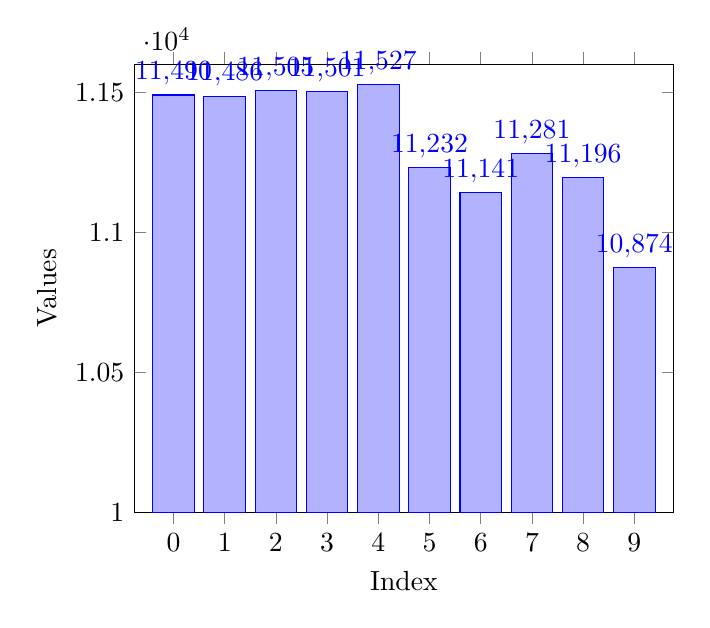
\begin{tikzpicture}
        \begin{axis}[
            ybar,
            bar width=15pt,
            ylabel={Values},
            xlabel={Index},
            xtick={0, 1, 2, 3, 4, 5, 6, 7, 8, 9},
            xticklabels={0, 1, 2, 3, 4, 5, 6, 7, 8, 9},
            nodes near coords,
            ymin=10000,
            ymax=11600,
            enlarge x limits={abs=0.5cm}
        ]
        \addplot coordinates {(0, 11490) (1, 11486) (2, 11505) (3, 11501) (4, 11527) (5, 11232) (6, 11141) (7, 11281) (8, 11196) (9, 10874)};
        \end{axis}
    \end{tikzpicture}
    \caption{Histogram danih podatkov}
    \label{fig:histogram}
\end{figure}

\section{Zaključek}

V zaključku bomo povzeli ugotovitve iz analize igre ustvarjanja omrežij, izpostavili ključne točke ter predlagali morebitne nadaljnje raziskave.

\end{document}
